% =============================================================================
% CHAPITRE 4 : ÉTUDE 1 - IMPACT DE L'INTERACTIVITÉ ET DE LA REPRÉSENTATION
% =============================================================================
% Structure alignée sur le modèle de thèse (sommaire + résumé + présentation)
% =============================================================================

\chapter{Étude 1 : Impact de l'Interactivité et de la Représentation sur l'Intérêt}
\label{ch:experimentation1}

% Sommaire de chapitre
\minitoc
\newpage

% =============================================================================
% SECTION 4.1 : RÉSUMÉ
% =============================================================================

\section{Résumé}
\label{sec:exp1-resume}

L'étude pilote exploratoire présentée au chapitre précédent a fourni des observations qualitatives encourageantes sur l'interaction orale avec des agents historiques virtuels, sans toutefois permettre d'isoler les mécanismes spécifiques à l'origine de ces réactions positives. Dans ce contexte, cette série de trois expérimentations vise à évaluer l'influence de deux facteurs sur l'intérêt des élèves pour le contenu historique : la modalité d'interaction (interactive vs. non-interactive) et l'alignement thématique entre l'identité de l'agent et le contenu pédagogique (figure historique vs. personnage neutre). Trois cent trente-neuf élèves répartis sur trois niveaux scolaires (6\textsuperscript{ème}, 4\textsuperscript{ème}, Terminale) ont participé à des sessions intégrées au programme d'histoire, interagissant avec des agents incarnant Napoléon Bonaparte, Jules César, Charles de Gaulle ou des personnages neutres/pairs. Nos résultats révèlent un effet robuste et consistant de l'interactivité : les élèves déclarent un intérêt significativement plus élevé pour l'activité d'apprentissage, le contenu de la leçon et le personnage historique dans les conditions interactives comparées aux présentations vidéo passives. L'effet de l'alignement thématique apparaît plus nuancé et dépendant du contexte. Aucun effet n'est observé avec Napoléon (4\textsuperscript{ème}), dont le style formel et autoritaire semble créer une distance avec les élèves. En revanche, Jules César, présenté de manière accessible et vulnérable, génère un intérêt supérieur au personnage neutre chez les élèves de 6\textsuperscript{ème}. Chez les lycéens de Terminale, aucune différence n'émerge entre la figure d'autorité (de Gaulle) et la figure de pair (Louis), suggérant que l'expertise perçue prime sur la similarité à cet âge. Ces résultats soulignent que l'efficacité des agents historiques virtuels dépend non seulement de l'interactivité, mais aussi de l'adéquation entre le style de présentation du personnage et le stade développemental des apprenants.


% =============================================================================
% SECTION 4.2 : PRÉSENTATION DE L'EXPÉRIMENTATION
% =============================================================================

\section{Présentation de l'expérimentation}
\label{sec:exp1-presentation}

Comme l'illustre notre revue de littérature, les sentiments de présence sociale et d'agentivité sont des composantes essentielles de l'expérience utilisateur dans les interactions avec des agents conversationnels (Chapitre~2). Nous avons dès lors identifié plusieurs facteurs susceptibles d'influencer l'intérêt des élèves pour le contenu pédagogique : l'interactivité, qui permet un dialogue bidirectionnel \citep{freeman2014active, deci2000intrinsic}, et l'alignement thématique entre l'identité de l'agent et le contenu de la leçon, qui pourrait activer des réponses sociales favorisant un traitement cognitif plus profond \citep{moreno2001, mayer2012}. L'identification des facteurs influençant l'intérêt des élèves constitue une étape essentielle afin de permettre le développement d'applications pédagogiques exploitant le potentiel des agents conversationnels historiques.

L'étendue des recherches actuelles permet d'identifier de nombreux facteurs affectant l'efficacité des agents pédagogiques \citep{hidi2006four, harackiewicz2016}. Cependant, les études portant sur la modalité d'interaction et ses conséquences sur l'intérêt divergent. Certaines démontrent que l'apprentissage actif serait la condition la plus appropriée pour induire un intérêt élevé \citep{freeman2014active, deslauriers2019}, tandis que d'autres n'observent pas de différences significatives entre les modalités passives et actives \citep{moreno2007interactive}. De plus, nous avons constaté que peu d'études analysent la relation entre l'alignement thématique d'un agent et l'intérêt des élèves en contexte scolaire authentique \citep{schmidt2019}. Ainsi, notre étude se propose de poursuivre les investigations nécessaires, notamment dans le cadre d'un cas d'usage proche de ce que l'industrie éducative pourrait proposer grâce à la démocratisation actuelle de l'IA générative.

Cette première série d'expérimentations menée dans le cadre de nos travaux de recherche ambitionne de déterminer l'impact de l'interactivité et de l'alignement thématique (Chapitre~2.4) sur l'intérêt des élèves en contexte scolaire. L'objectif consiste à évaluer l'influence des conditions interactives comparées aux présentations vidéo passives, ainsi que l'effet de la représentation d'une figure historique comparée à un personnage neutre, sur trois dimensions d'intérêt : l'intérêt pour l'activité d'apprentissage, l'intérêt pour le contenu de la leçon, et l'intérêt pour le personnage historique. Les résultats observés lors de ces études servent par ailleurs de support aux expérimentations subséquentes portant sur l'impact du design visuel des agents.

Le premier axe de cette expérimentation consiste à déterminer l'impact de l'interactivité sur l'intérêt des élèves. Dans ce contexte, l'utilisateur interagit soit avec un agent conversationnel en temps réel, soit visionne une présentation vidéo préenregistrée du même agent délivrant un contenu équivalent. L'évaluation subjective de l'intérêt repose sur des questionnaires adaptés de l'Inventaire de Motivation Intrinsèque \citep{deci1994facilitating}. Le deuxième axe de notre étude se focalise sur les implications relatives à l'alignement thématique concernant l'intérêt des élèves. Ces critères sont évalués en comparant des agents incarnant des figures historiques liées au contenu de la leçon à des agents neutres présentant le même contenu dans un style expositif.

Cette série comprend trois expérimentations distinctes, chacune ciblant un niveau scolaire différent et mobilisant un personnage historique spécifique. L'Expérimentation 1.1, menée avec des élèves de 4\textsuperscript{ème}, utilise Napoléon Bonaparte dans le cadre d'une leçon sur l'Empire français. L'Expérimentation 1.2, conduite avec des élèves de 6\textsuperscript{ème}, met en scène Jules César lors d'une séquence sur la République romaine. L'Expérimentation 1.3, réalisée avec des lycéens de Terminale, compare Charles de Gaulle à Louis, un jeune résistant fictif, dans le contexte de la Résistance française. Cette variation délibérée permet de tester la robustesse des effets observés à travers différents contextes développementaux.

La prochaine partie de ce chapitre présente successivement chaque expérimentation et l'ensemble de son protocole. Les résultats de chaque étude sont analysés dans leur section respective. Une discussion générale intègre les observations des trois études, préalablement à l'évocation des considérations éthiques communes et à la conclusion de cette première série expérimentale.


% =============================================================================
% SECTION 4.3 : EXPÉRIMENTATION 1.1 - L'EMPIRE FRANÇAIS (4ÈME)
% =============================================================================

\section{Expérimentation 1.1 : L'Empire Français avec des élèves de 4\textsuperscript{ème}}
\label{sec:exp11}

\subsection{Contexte Pédagogique}
\label{subsec:exp11-contexte}

Cette première étude a été intégrée au programme de 4\textsuperscript{ème} portant sur l'Empire Français. Nous avons examiné deux facteurs susceptibles d'influencer l'intérêt des élèves pour le contenu historique. Premièrement, nous avons comparé les présentations interactives et non interactives. Les présentations vidéo non interactives offrent un contenu visuel et des éléments narratifs qui diffèrent des cours magistraux traditionnels. Les conditions interactives permettent aux élèves de dialoguer avec un agent virtuel, de poser des questions et de recevoir des réponses immédiates. Deuxièmement, nous avons examiné l'effet de l'alignement du personnage en comparant des agents historiques et neutres dans les conditions interactives et non interactives. Cette approche nous a permis d'étudier si l'alignement entre l'identité de l'agent et le contenu historique influence l'intérêt des élèves. Basée sur un plan expérimental inter-sujets, cette étude a mis en œuvre des conditions en classe pour maintenir la validité écologique.

\subsection{Conditions Expérimentales}
\label{subsec:exp11-conditions}

L'étude a employé un plan 2×2 inter-sujets avec deux variables indépendantes : l'Interactivité (Interactive vs. Non-Interactive) et l'alignement du personnage (Historique vs. Neutre). En utilisant Napoléon Bonaparte comme personnage historique, nous avons mesuré les effets de l'interactivité et de l'alignement du personnage sur trois dimensions d'intérêt : l'intérêt pour l'activité d'apprentissage, la figure historique et le contenu de la leçon. 

Dans les conditions interactives, les élèves ont participé à une conversation ouverte de 10 minutes avec l'agent virtuel généré par IA. L'agent a répondu aux questions, fourni des réponses contextuellement pertinentes et utilisé des expressions faciales et un ton vocal synchronisés pour transmettre des émotions. Dans les conditions non interactives, les élèves ont regardé une vidéo pré-enregistrée de 10 minutes de l'agent délivrant un monologue, avec des expressions faciales et un ton vocal synchronisés.

Pour l'alignement du personnage, la condition historique mettait en scène Napoléon Bonaparte parlant à la première personne, partageant des anecdotes personnelles et des expériences. La condition neutre, en revanche, présentait les mêmes informations historiques à travers un agent utilisant un style expositif, parlant à la troisième personne sans embellissement historique et utilisant des expressions plus sobres (voir Figure~\ref{fig:napoleon_conditions}).

\begin{figure}[htbp]
    \centering
    \includegraphics[width=0.8\textwidth]{images/ch4/napoleon_conditions.png}
    \caption{Comparaison des agents virtuels dans les conditions historique (Napoléon Bonaparte) et neutre de l'Expérimentation 1.1}
    \label{fig:napoleon_conditions}
\end{figure}

\subsection{Équipement}
\label{subsec:exp11-equipement}

L'expérience s'est déroulée dans des salles de classe régulières, chacune équipée d'un ordinateur portable positionné sur le bureau de l'enseignant pour exécuter le système MemorIA. L'ordinateur portable, un Dell Precision 7780 avec un processeur Intel Core i7-1185G7, une carte graphique NVIDIA RTX 4090, 16 Go de RAM, avait deux dispositifs connectés : un haut-parleur de conférence Jabra Speak 750 pour capturer les demandes verbales des élèves, et une connexion au système d'affichage de la classe. Cette configuration permettait à toute la classe de voir et d'entendre simultanément l'agent virtuel pendant les sessions interactives. Pour les conditions non interactives, des vidéos pré-enregistrées ont été diffusées sur le même système. La taille de l'image projetée a été maintenue constante à travers les trois études, assurant la cohérence dans la présentation visuelle des agents virtuels.

\subsection{Participants}
\label{subsec:exp11-participants}

L'étude a impliqué un échantillon de 113 élèves de 4\textsuperscript{ème} (59 filles, 54 garçons ; âge : M = 13,2 ans, ET = 0,8, étendue : 12-14 ans) recrutés dans un collège français. Les participants ont été recrutés dans quatre classes, résultant en environ 30 élèves par classe.

Le protocole d'étude a été examiné et approuvé par le comité d'éthique institutionnel. Les parents et les élèves ont reçu des informations détaillées sur l'étude et ont été informés que la participation était volontaire. Un consentement écrit a été obtenu des parents/tuteurs légaux, et les élèves ont fourni un assentiment écrit. Seuls les élèves ayant retourné les deux formulaires ont participé à l'expérience. Tout au long du processus, les participants ont été assurés de leur droit à la confidentialité et de leur liberté de se retirer de l'étude.

\subsection{Procédure}
\label{subsec:exp11-procedure}

L'expérience a été intégrée dans une leçon d'histoire régulière de 60 minutes dans des conditions « écologiques » authentiques. En arrivant dans la salle de classe, l'enseignant a accueilli et présenté les expérimentateurs aux élèves. Après que les expérimentateurs ont expliqué les activités prévues, tous les participants ont complété un questionnaire initial évaluant leur intérêt pour l'activité d'apprentissage, la figure historique et le contenu de la leçon. 

Les classes ont été assignées aléatoirement à l'une des quatre conditions expérimentales. Dans les conditions interactives, les élèves ont été informés qu'ils interagiraient avec un agent virtuel, représentant soit une figure historique soit un personnage neutre. Les élèves ont travaillé en petits groupes de 3-4 pour générer collaborativement des questions liées au sujet de la leçon. Chaque groupe a sélectionné un porte-parole qui s'est engagé avec l'agent virtuel (personnifiant soit Napoléon Bonaparte soit un personnage neutre) pendant environ 2 minutes. Les réponses parlées de l'agent, accompagnées d'expressions faciales appropriées, ont été affichées sur un grand écran avec l'audio diffusé à travers les haut-parleurs de la classe, permettant à toute la classe d'observer chaque interaction.

Dans les conditions non interactives, les participants ont visionné une vidéo pré-enregistrée de 10 minutes de l'agent virtuel (figure historique ou neutre) délivrant un monologue sur sa vie et ses expériences, se concentrant sur des sujets liés au contenu de la leçon (voir Figure~\ref{fig:classroom_napoleon}).

\begin{figure}[htbp]
    \centering
    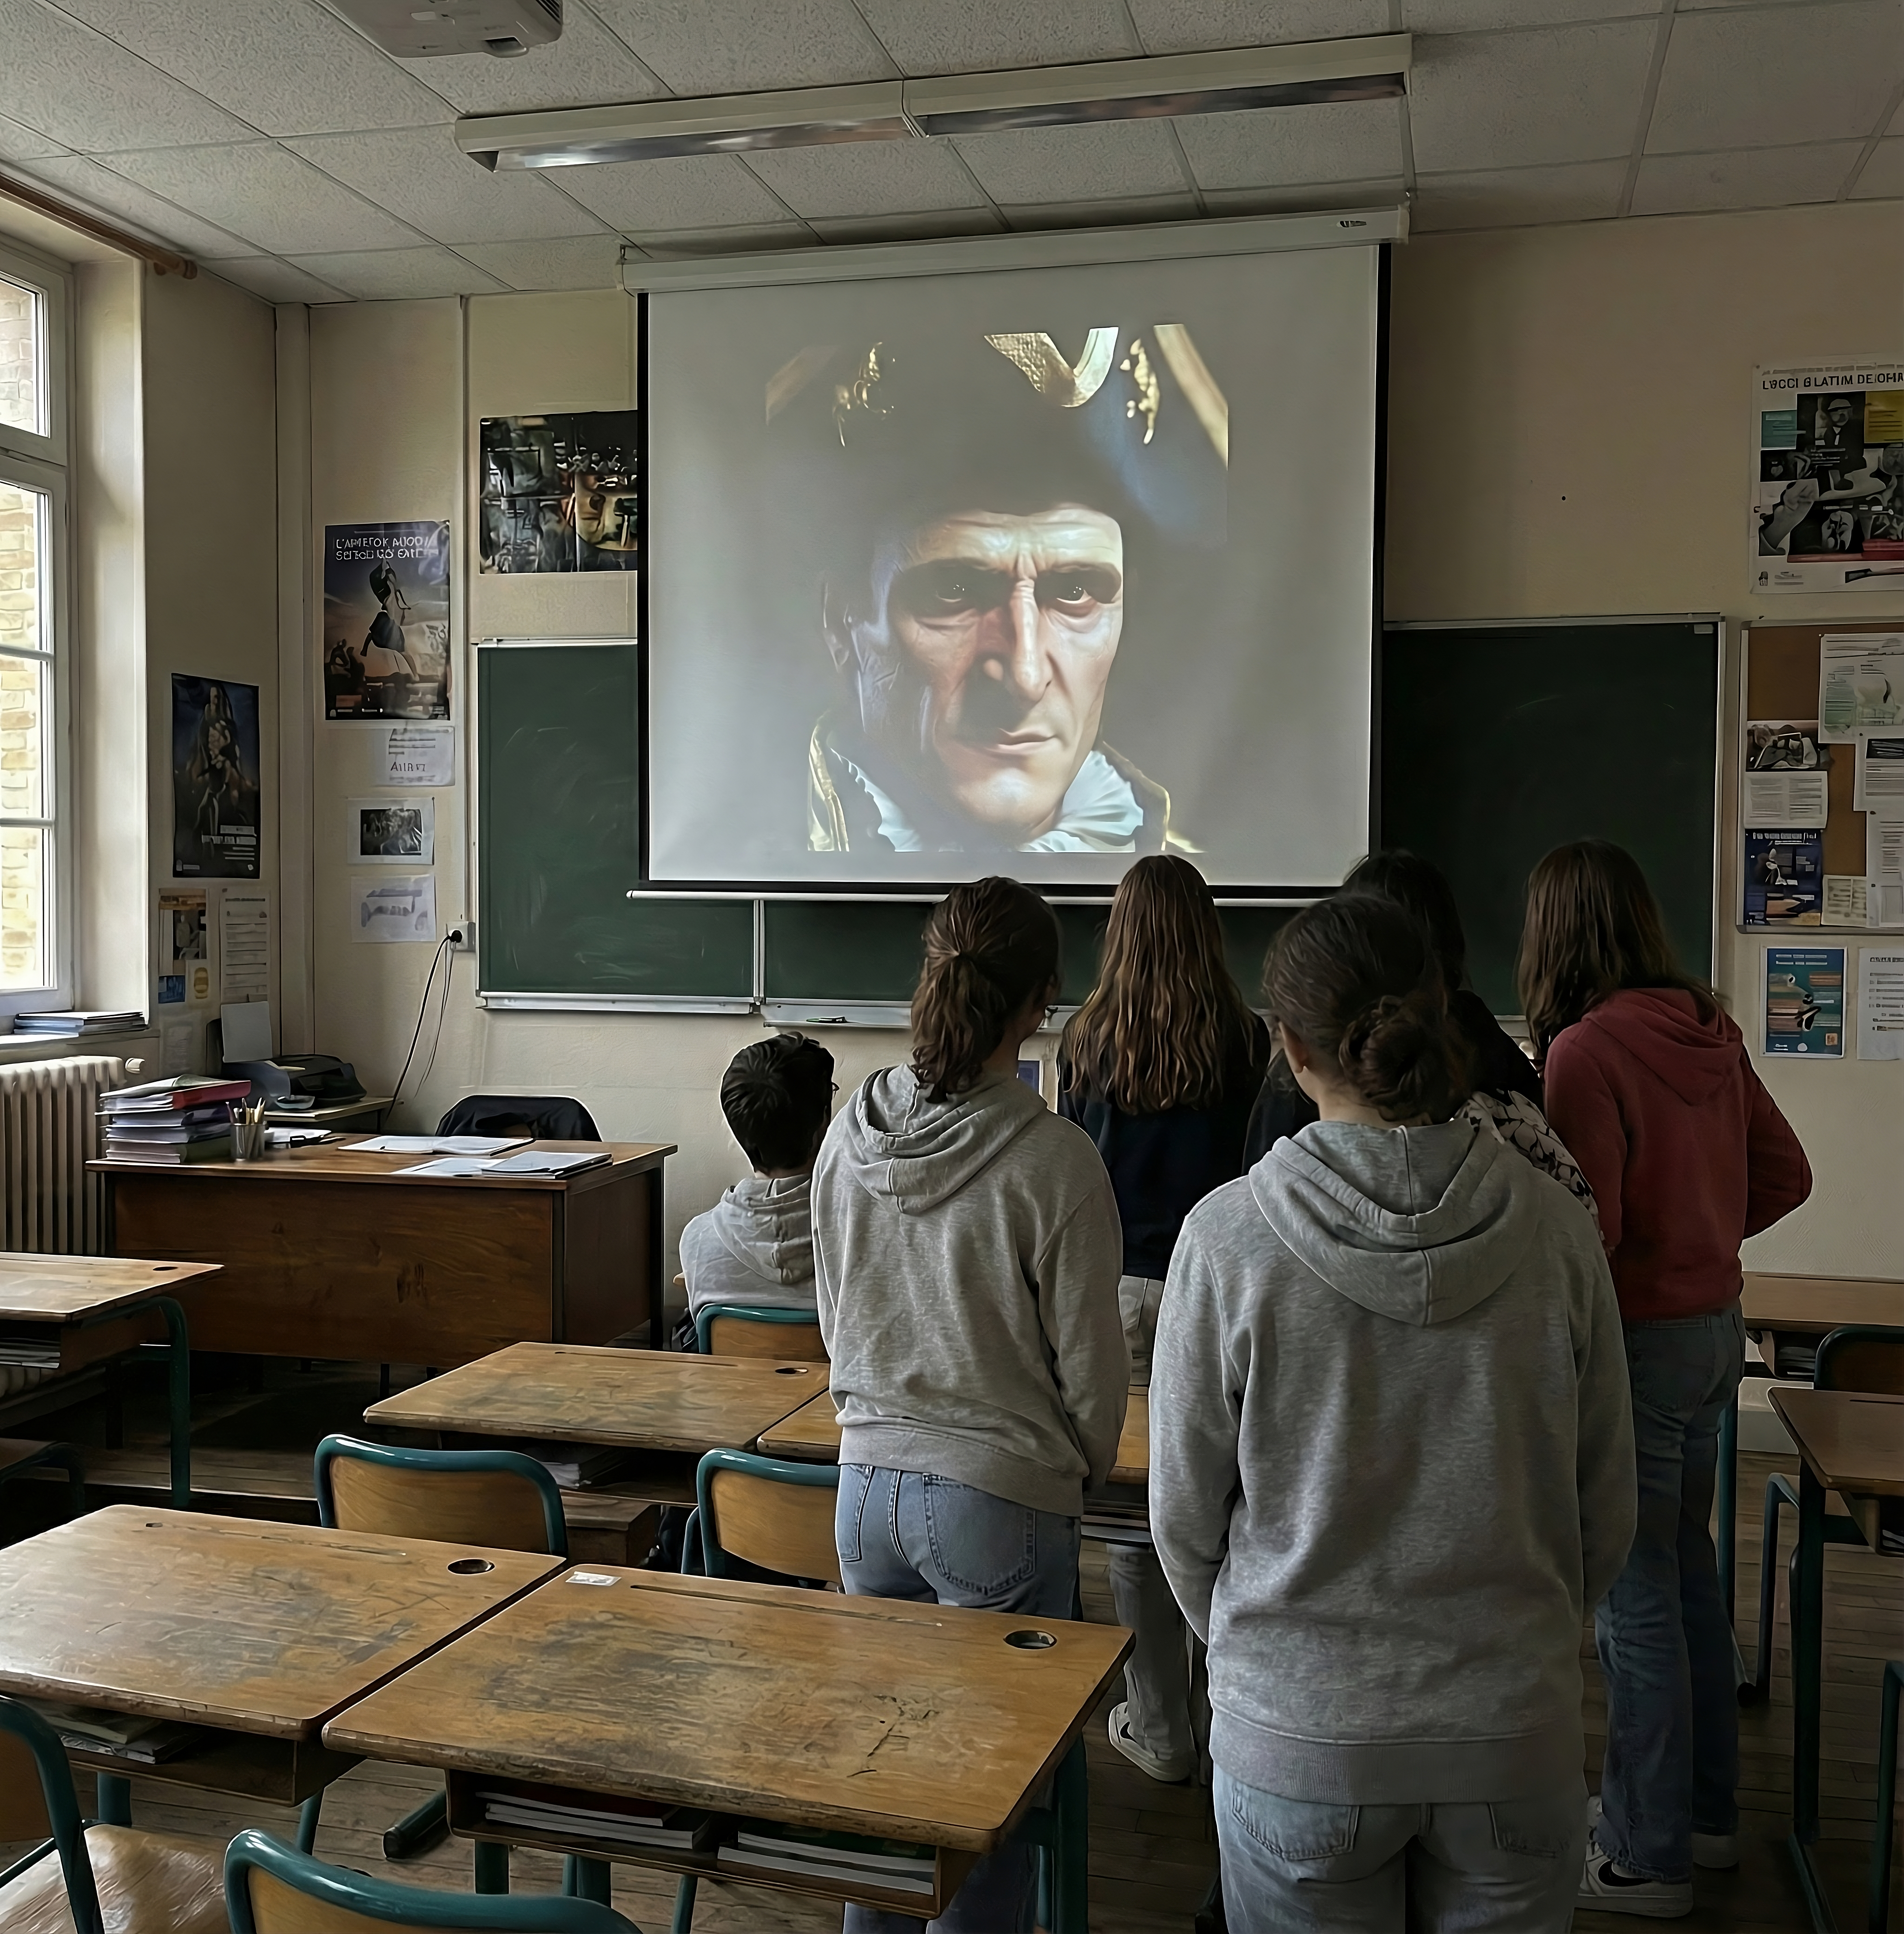
\includegraphics[width=0.8\textwidth]{images/ch4/classroom_napoleon.png}
    \caption{Configuration de la classe pendant l'Expérimentation 1.1 avec Napoléon Bonaparte}
    \label{fig:classroom_napoleon}
\end{figure}

Suite à la phase expérimentale, les participants ont complété un questionnaire post-expérience évaluant les mêmes trois dimensions d'intérêt. Des discussions de groupe ont ensuite été facilitées avec chaque classe, fournissant un forum ouvert pour que les participants partagent leurs réflexions sur leurs interactions avec les agents virtuels. Nous avons souligné que les agents virtuels étaient des représentations générées par IA, et l'enseignant a eu l'opportunité de clarifier et de corriger toute inexactitude historique qui a émergé pendant les interactions. Au cours de ces discussions, les participants ont exploré des questions sur l'authenticité historique et les implications de l'utilisation de l'IA dans des contextes éducatifs.

\subsection{Mesures}
\label{subsec:exp11-mesures}

L'intérêt a été évalué à l'aide de questionnaires adaptés de l'Inventaire de Motivation Intrinsèque (IMI) \citep{deci1994facilitating} et alignés avec les travaux de \citet{hidi2006four} sur le développement de l'intérêt situationnel et individuel.

Trois dimensions ont été mesurées : l'intérêt pour l'activité d'apprentissage (plaisir, valeur et volonté de s'engager), l'intérêt pour la figure historique (curiosité et désir d'en apprendre davantage sur le personnage), et l'intérêt pour le contenu de la leçon (engagement et curiosité concernant l'Empire Français). Chaque dimension a été évaluée à travers trois items distincts de questionnaire. Les questions ont été notées sur des échelles à 7 points allant de 1 (fortement en désaccord) à 7 (fortement en accord). Pour minimiser les effets d'ordre et les biais de réponse, les items ont été entièrement randomisés à travers toutes les dimensions. Les réponses au questionnaire pré-expérience, mesurant l'intérêt initial pour l'activité d'apprentissage, la figure historique et le contenu de la leçon, ont été utilisées comme covariables dans les analyses pour contrôler les différences individuelles dans l'intérêt de base.

\subsection{Hypothèses}
\label{subsec:exp11-hypotheses}

Basées sur notre revue de la littérature et le design de notre étude, nous avons proposé les hypothèses suivantes :

\textbf{H1 :} Les participants dans les conditions interactives présenteront un intérêt post-intervention plus élevé pour l'activité d'apprentissage (H1.1), le contenu de la leçon (H1.2), et le personnage historique (H1.3) comparé à ceux dans les conditions non interactives, après contrôle des niveaux d'intérêt pré-intervention.

Cette hypothèse est fondée sur les bénéfices pédagogiques établis de l'apprentissage actif et de l'interactivité \citep{freeman2014active, moreno2007interactive}. L'engagement des élèves, facilité par le dialogue et le contrôle du rythme d'apprentissage, est suggéré comme étant un facteur clé dans la promotion de la motivation intrinsèque et de l'apprentissage profond \citep{deci2000intrinsic}. Des recherches récentes indiquent que les interactions conversationnelles avec des agents pédagogiques peuvent améliorer significativement l'engagement et l'intérêt des apprenants \citep{hidi2006four}. L'impact positif des agents virtuels interactifs alimentés par l'IA sur divers résultats d'apprentissage \citep{pataranutaporn2023, prasongpongchai2024} s'aligne avec les théories de l'apprentissage multimédia mettant l'accent sur l'importance de la communication bidirectionnelle pour un traitement cognitif efficace \citep{moreno2007interactive}.

\textbf{H2 :} Les participants dans les conditions de figure historique présenteront un intérêt post-intervention plus élevé pour l'activité d'apprentissage (H2.1), le contenu de la leçon (H2.2), et le personnage historique (H2.3) comparé à ceux dans les conditions de figure neutre, après contrôle des niveaux d'intérêt pré-intervention.

Cette hypothèse est basée sur la théorie de l'agence sociale \citep{moreno2001, mayer2012}, qui postule que les signaux sociaux dans les environnements d'apprentissage peuvent activer des réponses sociales chez les apprenants, conduisant à un traitement cognitif plus profond. La représentation de figure historique peut influencer l'intérêt des élèves par deux mécanismes : premièrement, en impliquant l'interaction avec des personnalités célèbres et potentiellement admirées \citep{pataranutaporn2022}, et deuxièmement, par l'alignement thématique entre la figure historique et le contenu de la leçon \citep{schmidt2019}.

\subsection{Résultats}
\label{subsec:exp11-resultats}

Nous avons conduit des analyses de covariance bidirectionnelles (ANCOVA) pour chaque variable dépendante (intérêt pour l'activité d'apprentissage [Post\_Act], intérêt pour le contenu de la leçon [Post\_Les], et intérêt pour le personnage historique [Post\_Char]), avec l'interactivité et l'alignement du personnage comme variables indépendantes et les mesures pré-intervention correspondantes comme covariables. Cette approche nous a permis de contrôler les différences préexistantes entre les participants tout en testant nos hypothèses sur les effets de l'interactivité et de l'alignement du personnage sur l'intérêt des élèves.

Avant d'analyser les effets de nos variables indépendantes, nous avons vérifié la comparabilité initiale des groupes expérimentaux. Des tests de Mann-Whitney ont comparé les scores d'intérêt initiaux entre les conditions d'interactivité (Vidéo vs. Interactive) et d'alignement du personnage (Neutre vs. Historique). Aucune différence significative n'a été trouvée entre les groupes, démontrant une bonne comparabilité initiale.

Aucun effet d'interaction significatif entre l'interactivité et l'alignement du personnage n'a été observé pour aucune des mesures d'intérêt (Post\_Act : F(1, 108) = 1,399, p = ,240, $\eta^2$ = ,010 ; Post\_Les : F(1, 108) = 0,457, p = ,501, $\eta^2$ = ,002 ; Post\_Char : F(1, 108) = 1,336, p = ,250, $\eta^2$ = ,007). 

Un effet principal de l'interactivité a été observé sur l'intérêt pour l'activité d'apprentissage (Post\_Act ; F(1, 108) = 23,547, p < ,001, $\eta^2$ = ,166), tandis que l'alignement du personnage n'a montré aucun effet significatif (F(1, 108) = 2,269, p = ,135, $\eta^2$ = ,016). Les élèves dans les conditions interactives ont rapporté un intérêt plus élevé (M = 5,699, ET = 1,133 pour le personnage historique ; M = 5,844, ET = 1,176 pour le personnage neutre) comparé à ceux dans les conditions vidéo (M = 4,226, ET = 1,513 pour le personnage historique ; M = 4,960, ET = 1,338 pour le personnage neutre).

\begin{figure}[htbp]
    \centering
    \includegraphics[width=0.6\textwidth]{images/ch4/napoleon_post_act.png}
    \caption{Intérêt des élèves de 4\textsuperscript{ème} pour l'activité d'apprentissage (Post\_Act) en fonction de l'interactivité et de l'alignement du personnage. Les barres d'erreur représentent les écarts-types}
    \label{fig:napoleon_post_act}
\end{figure}

Pour l'intérêt pour le contenu de la leçon (Post\_Les), un effet principal de l'interactivité a été trouvé (F(1, 108) = 11,231, p = ,001, $\eta^2$ = ,052), sans effet significatif de l'alignement du personnage (F(1, 108) = 1,377, p = ,243, $\eta^2$ = ,006).

\begin{figure}[htbp]
    \centering
    \includegraphics[width=0.6\textwidth]{images/ch4/napoleon_post_les.png}
    \caption{Intérêt des élèves de 4\textsuperscript{ème} pour le contenu de la leçon (Post\_Les) en fonction de l'interactivité et de l'alignement du personnage. Les barres d'erreur représentent les écarts-types}
    \label{fig:napoleon_post_les}
\end{figure}

De manière similaire, pour l'intérêt pour le personnage historique (Post\_Char), l'analyse a révélé un effet principal de l'interactivité (F(1, 108) = 5,901, p = ,017, $\eta^2$ = ,030), sans effet significatif de l'alignement du personnage (F(1, 108) = 0,337, p = ,563, $\eta^2$ = ,002).

\begin{figure}[htbp]
    \centering
    \includegraphics[width=0.6\textwidth]{images/ch4/napoleon_post_char.png}
    \caption{Intérêt des élèves de 4\textsuperscript{ème} pour le personnage historique (Post\_Char) en fonction de l'interactivité et de l'alignement du personnage. Les barres d'erreur représentent les écarts-types}
    \label{fig:napoleon_post_char}
\end{figure}

\subsection{Discussion}
\label{subsec:exp11-discussion}

Notre analyse a révélé des patterns spécifiques concernant les effets de l'interactivité sur l'intérêt des élèves, tandis que l'alignement du personnage n'a montré aucune influence claire. Pour notre première hypothèse (H1), l'interactivité a démontré une influence positive significative sur l'intérêt des élèves. Les élèves qui participent à des dialogues avec des agents virtuels rapportent des niveaux d'intérêt plus élevés pour l'activité d'apprentissage, le contenu de la leçon et le personnage historique comparés à ceux qui visionnent des vidéos non interactives. Ces résultats s'alignent avec la recherche sur les interactions avec des agents virtuels alimentés par l'IA \citep{prasongpongchai2024, pataranutaporn2023}.

Notre seconde hypothèse (H2) prédisait un intérêt plus élevé pour le personnage historique, mais les données n'ont révélé aucune différence significative. Alors que des recherches antérieures suggéraient des bénéfices de l'alignement thématique pour l'intérêt dans les interactions virtuelles, nos résultats indiquent qu'un tel alignement nécessite des considérations additionnelles pour favoriser efficacement l'intérêt. Les retours qualitatifs révèlent que les élèves ont perçu la narration de Napoléon comme distante, caractérisée par un langage formel qui a créé des barrières plutôt que des opportunités de connexion. Le personnage neutre, non contraint par une telle formalité, semble fournir un point d'entrée plus accessible au contenu. Cela s'aligne avec la recherche de \citet{lin2020} mettant en évidence comment le style conversationnel peut impacter significativement l'intérêt dans des contextes éducatifs.


% =============================================================================
% SECTION 4.4 : EXPÉRIMENTATION 1.2 - L'EMPIRE ROMAIN (6ÈME)
% =============================================================================

\section{Expérimentation 1.2 : L'Empire Romain avec des élèves de 6\textsuperscript{ème}}
\label{sec:exp12}

\subsection{Contexte Pédagogique et Choix du Personnage}
\label{subsec:exp12-contexte}

En réponse aux observations de la première étude, nous avons apporté des modifications importantes à notre approche pour l'étude suivante avec des élèves de 6\textsuperscript{ème}. Nous avons sélectionné Jules César comme figure historique en raison de sa forte présence dans la culture populaire française, notamment à travers les bandes dessinées Astérix. Les élèves de 6\textsuperscript{ème} (10-12 ans) sont familiers avec César à travers ces médias, potentiellement créant une connexion plus accessible que Napoléon pour les élèves de 4\textsuperscript{ème}. 

De plus, nous avons adapté le style de présentation et le conditionnement du personnage de César pour créer une persona plus empathique et accessible. Contrairement au ton formel et autoritaire de Napoléon, le personnage de César a été développé avec :

\begin{itemize}
\item Un accent sur la vulnérabilité et les expériences personnelles
\item Des reconnaissances de doutes et d'anxiétés
\item Un style conversationnel décontracté, avec des blagues occasionnelles et des réponses ludiques
\end{itemize}

\subsection{Conditions Expérimentales et Plan}
\label{subsec:exp12-conditions}

Le plan expérimental a reflété celui de l'Étude 1, employant un plan inter-sujets 2×2 avec les mêmes variables indépendantes : Interactivité (Interactive vs. Non-Interactive) et alignement du personnage (Historique vs. Neutre). Les quatre conditions expérimentales étaient identiques à la première étude, Jules César remplaçant Napoléon Bonaparte (voir Figure~\ref{fig:caesar_conditions}).

\begin{figure}[htbp]
    \centering
    \includegraphics[width=0.8\textwidth]{images/ch4/caesar_conditions.png}
    \caption{Comparaison des agents virtuels dans les conditions historique (Jules César) et neutre de l'Expérimentation 1.2}
    \label{fig:caesar_conditions}
\end{figure}

\subsection{Participants}
\label{subsec:exp12-participants}

La deuxième étude a impliqué un échantillon de 113 élèves de 6\textsuperscript{ème} (61 filles, 52 garçons ; âge : M = 11,2 ans, ET = 0,7, étendue : 10-12 ans) recrutés dans le même collège français. L'étude a suivi les mêmes directives éthiques que la première étude, assurant la participation volontaire et le consentement éclairé des élèves et de leurs parents/tuteurs.

\subsection{Procédure}
\label{subsec:exp12-procedure}

L'expérience a suivi le protocole de l'Étude 1. L'expérience s'est déroulée dans le cadre d'une seule leçon d'histoire de 60 minutes. Les participants ont d'abord complété un questionnaire initial évaluant leur intérêt pour le sujet de la leçon (la Guerre des Gaules), la figure historique (Jules César ou personnage neutre), et l'activité d'apprentissage. Les classes ont été assignées aléatoirement à l'une des quatre conditions expérimentales.

\begin{figure}[htbp]
    \centering
    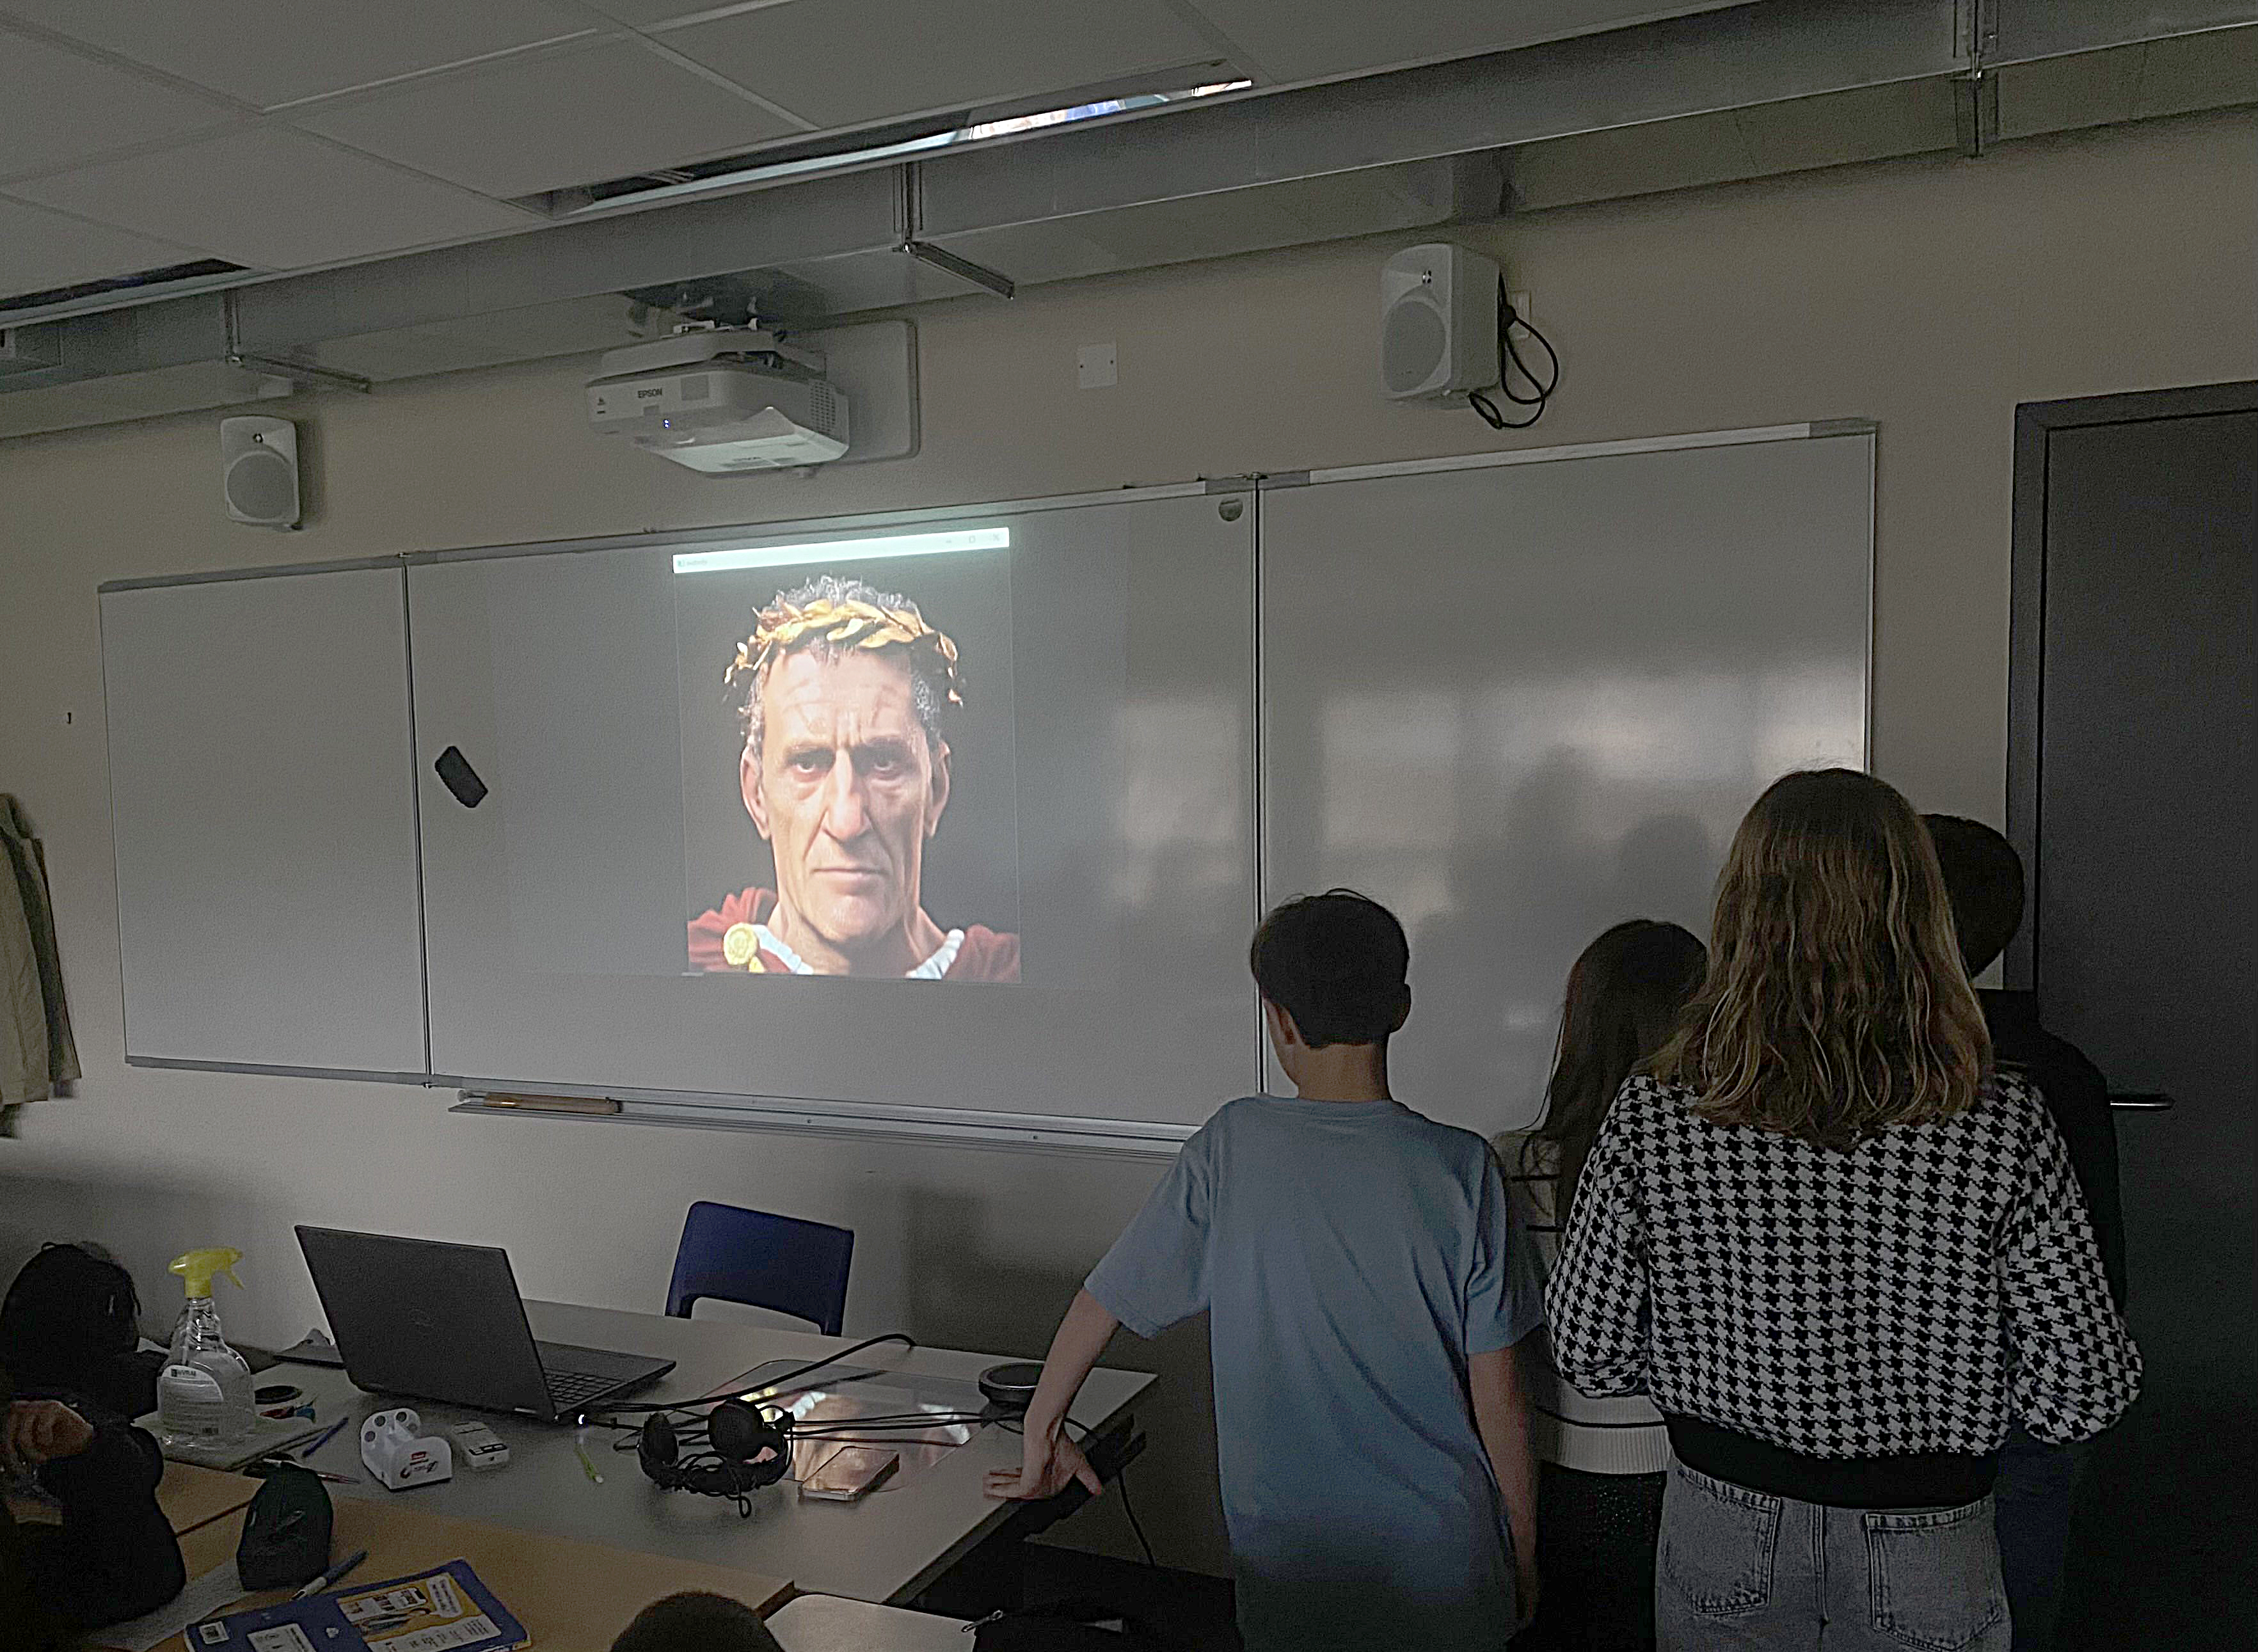
\includegraphics[width=0.8\textwidth]{images/ch4/classroom_caesar.png}
    \caption{Élèves de 6\textsuperscript{ème} interagissant avec Jules César pendant l'Expérimentation 1.2}
    \label{fig:classroom_caesar}
\end{figure}

\subsection{Mesures et Hypothèses}
\label{subsec:exp12-mesures}

Les mesures d'intérêt ont été maintenues cohérentes avec l'Étude 1, utilisant des questionnaires adaptés de l'IMI \citep{deci1994facilitating}. Pour l'Étude 2, nous avons maintenu les hypothèses concernant les effets de l'interactivité (H1) et de l'alignement du personnage (H2) sur l'intérêt des élèves.

\subsection{Résultats}
\label{subsec:exp12-resultats}

Les ANCOVA n'ont révélé aucun effet d'interaction significatif entre l'interactivité et l'alignement du personnage pour Post\_Act (F(1, 108) = 2,505, p = ,116, $\eta^2$ = ,011), Post\_Les (F(1, 108) = 3,027, p = ,085, $\eta^2$ = ,011), ou Post\_Char (F(1, 108) = 2,043, p = ,156, $\eta^2$ = ,008).

Pour l'intérêt pour l'activité d'apprentissage (Post\_Act ; voir Figure~\ref{fig:caesar_post_act}), un effet principal de l'interactivité a été observé (F(1, 108) = 76,58, p < ,001, $\eta^2$ = ,330), avec des participants dans les conditions interactives rapportant un intérêt plus élevé. Un effet principal de l'alignement du personnage a également été trouvé (F(1, 108) = 11,425, p = ,001, $\eta^2$ = ,049).

\begin{figure}[htbp]
    \centering
    \includegraphics[width=0.6\textwidth]{images/ch4/caesar_post_act.png}
    \caption{Intérêt des élèves de 6\textsuperscript{ème} pour l'activité d'apprentissage (Post\_Act) en fonction de l'interactivité et de l'alignement du personnage}
    \label{fig:caesar_post_act}
\end{figure}

Pour l'intérêt pour le contenu de la leçon (Post\_Les), un effet principal de l'interactivité a été trouvé (F(1, 108) = 52,118, p < ,001, $\eta^2$ = ,187). Un effet principal de l'alignement du personnage a également été observé (F(1, 108) = 15,603, p < ,001, $\eta^2$ = ,056).

\begin{figure}[htbp]
    \centering
    \includegraphics[width=0.6\textwidth]{images/ch4/caesar_post_les.png}
    \caption{Intérêt des élèves de 6\textsuperscript{ème} pour le contenu de la leçon (Post\_Les) en fonction de l'interactivité et de l'alignement du personnage}
    \label{fig:caesar_post_les}
\end{figure}

Concernant l'intérêt pour le personnage historique (Post\_Char), un effet principal de l'interactivité a été trouvé (F(1, 108) = 47,261, p < ,001, $\eta^2$ = ,174). Un effet principal de l'alignement du personnage a également été observé (F(1, 108) = 10,048, p = ,002, $\eta^2$ = ,037).

\begin{figure}[htbp]
    \centering
    \includegraphics[width=0.6\textwidth]{images/ch4/caesar_post_char.png}
    \caption{Intérêt des élèves de 6\textsuperscript{ème} pour le personnage historique (Post\_Char) en fonction de l'interactivité et de l'alignement du personnage}
    \label{fig:caesar_post_char}
\end{figure}

\subsection{Discussion}
\label{subsec:exp12-discussion}

L'analyse des données de l'étude avec les élèves de 6\textsuperscript{ème} améliore notre compréhension de l'influence des caractéristiques des agents virtuels sur l'intérêt des élèves. Conformément à notre première hypothèse (H1), l'interactivité a eu un effet positif sur l'intérêt des élèves pour les trois dimensions mesurées. Concernant notre seconde hypothèse (H2), nos résultats diffèrent de ceux de l'Étude 1. Alors que la présentation formelle de Napoléon semble créer des barrières avec les élèves de 4\textsuperscript{ème}, Jules César génère plus d'intérêt que le personnage neutre parmi les élèves de 6\textsuperscript{ème}.

Cette différence peut provenir de plusieurs facteurs interdépendants. Dans leur étude, \citet{linsiegler2016} ont montré que présenter les difficultés intellectuelles rencontrées par des scientifiques célèbres, incluant la faillibilité et l'auto-divulgation, permet une connexion avec l'agent. Le contexte développemental des élèves pourrait également influencer les résultats. Les élèves de 6\textsuperscript{ème} montrent une plus grande ouverture à l'engagement imaginatif \citep{brown2009}, combinée à leur inclinaison naturelle vers l'émerveillement \citep{prade2022}.


% =============================================================================
% SECTION 4.5 : EXPÉRIMENTATION 1.3 - LA RÉSISTANCE (TERMINALE)
% =============================================================================

\section{Expérimentation 1.3 : La Résistance avec des élèves de Terminale}
\label{sec:exp13}

\subsection{Contexte Pédagogique et Évolution du Plan Expérimental}
\label{subsec:exp13-contexte}

Cette troisième étude, ciblant des lycéens de Terminale, a examiné l'effet de l'alignement du personnage dans un contexte de développement cognitif plus avancé. Basée sur les résultats des études précédentes montrant des effets robustes de l'interactivité, nous avons simplifié le plan expérimental pour nous concentrer uniquement sur les conditions interactives. Nous avons comparé deux types de personnages : Charles de Gaulle comme figure historique d'autorité, et « Louis », un jeune combattant de la Résistance française, comme figure de pair.

\subsection{Développement des Personnages}
\label{subsec:exp13-personnages}

Le personnage de Charles de Gaulle a été développé pour incarner une figure d'autorité avec un conditionnement de personnage formel. Le personnage de « Louis », en revanche, a été conçu comme un jeune adulte (environ 20 ans) pour servir de figure de pair. Pour la représentation virtuelle de de Gaulle, nous avons utilisé Midjourney V5 pour générer un portrait. Sa voix a été recréée en utilisant la fonctionnalité de clonage vocal d'ElevenLabs entraînée sur des enregistrements de discours historiques. Le design du personnage de Louis a été développé en utilisant le Mode Remix de Midjourney V6.

\subsection{Conditions Expérimentales}
\label{subsec:exp13-conditions}

L'Étude 3 a employé un plan expérimental simplifié avec deux conditions :

\begin{itemize}
\item \textbf{Personnage Historique :} Les participants ont interagi avec Charles de Gaulle
\item \textbf{Personnage Pair :} Les participants ont interagi avec Louis
\end{itemize}

\begin{figure}[htbp]
    \centering
    \includegraphics[width=0.8\textwidth]{images/ch4/degaulle_louis_comparison.png}
    \caption{Comparaison des conditions Personnage Historique (Charles de Gaulle) et Personnage Pair (Louis)}
    \label{fig:degaulle_louis}
\end{figure}

\subsection{Participants}
\label{subsec:exp13-participants}

L'Étude 3 a impliqué un échantillon de 113 lycéens de Terminale (48 filles, 65 garçons ; âge : M = 17,45 ans, ET = 0,694, étendue : 16,0-19,0 ans).

\subsection{Procédure et Mesures}
\label{subsec:exp13-procedure}

L'expérience a suivi la même procédure que les études précédentes. L'intérêt a été évalué à l'aide de questionnaires adaptés de l'IMI \citep{deci1994facilitating}.

\subsection{Hypothèses}
\label{subsec:exp13-hypotheses}

Nous avons émis l'hypothèse que l'âge similaire, l'apparence et le style de communication de Louis pourraient favoriser une identification sociale plus forte que la figure historique plus distante de de Gaulle.

\textbf{H1 :} Les participants interagissant avec le personnage pair (Louis) rapporteront des niveaux d'intérêt plus élevés pour l'activité d'apprentissage (H1.1), le contenu de la leçon (H1.2), et le personnage historique (H1.3) comparés à ceux interagissant avec la figure historique (Charles de Gaulle).

\subsection{Résultats}
\label{subsec:exp13-resultats}

Les ANCOVA n'ont révélé aucun effet significatif du type de personnage sur l'intérêt pour l'activité (Post\_Act ; F(1, 110) = 0,057, p = ,812, $\eta^2$ = ,0003). L'intérêt pré-intervention (Pre\_Act) est apparu comme un prédicteur significatif (F(1, 110) = 78,359, p < ,001, $\eta^2$ = ,408).

\begin{figure}[htbp]
    \centering
    \includegraphics[width=0.6\textwidth]{images/ch4/degaulle_louis_post_act.png}
    \caption{Intérêt des lycéens de Terminale pour l'activité (Post\_Act) en fonction du type de personnage}
    \label{fig:degaulle_louis_post_act}
\end{figure}

Pour le contenu de la leçon (Post\_Les), l'analyse n'a montré aucun effet significatif du type de personnage (F(1, 110) = 1,330, p = ,251, $\eta^2$ = ,005).

\begin{figure}[htbp]
    \centering
    \includegraphics[width=0.6\textwidth]{images/ch4/degaulle_louis_post_les.png}
    \caption{Intérêt des lycéens de Terminale pour le contenu de la leçon (Post\_Les) en fonction du type de personnage}
    \label{fig:degaulle_louis_post_les}
\end{figure}

Pour l'intérêt pour le personnage (Post\_Char), aucun effet significatif du type de personnage n'a été observé (F(1, 110) = 0,555, p = ,458, $\eta^2$ = ,002).

\begin{figure}[htbp]
    \centering
    \includegraphics[width=0.6\textwidth]{images/ch4/degaulle_louis_post_char.png}
    \caption{Intérêt des lycéens de Terminale pour le personnage (Post\_Char) en fonction du type de personnage}
    \label{fig:degaulle_louis_post_char}
\end{figure}

\subsection{Discussion}
\label{subsec:exp13-discussion}

Contrairement à nos hypothèses (H1), l'interaction avec Louis n'a pas généré plus d'intérêt que l'interaction avec de Gaulle parmi les lycéens de Terminale. L'absence de différence significative est particulièrement notable lorsqu'on la compare à l'intérêt élevé observé chez les élèves de 6\textsuperscript{ème} ayant interagi avec César.

Une explication possible réside dans le développement d'une perspective critique sur la technologie parmi les lycéens. L'étude de \citet{nguyen2022-hm} sur l'évolution des perceptions des agents conversationnels avec l'âge corrobore cette idée. Les lycéens pourraient percevoir les tentatives de créer un lien artificiel à travers la similarité avec un personnage de type pair comme superficielles. L'expertise perçue, plus que la simple similarité, serait alors cruciale pour susciter l'intérêt à cet âge.


% =============================================================================
% SECTION 4.6 : DISCUSSION GÉNÉRALE
% =============================================================================

\section{Discussion générale}
\label{sec:exp1-discussion-generale}

\subsection{Synthèse des résultats}
\label{subsec:exp1-synthese}

Les trois expérimentations présentées dans ce chapitre permettent de dégager plusieurs constats. L'effet de l'interactivité s'avère robuste et consistant à travers les contextes : les élèves, quel que soit leur niveau scolaire, déclarent un intérêt significativement plus élevé lorsqu'ils peuvent dialoguer avec l'agent plutôt que de visionner une présentation vidéo passive. L'effet de l'alignement thématique apparaît plus nuancé et dépendant du contexte développemental et du style de présentation du personnage.

\subsection{Implications pour la conception d'agents pédagogiques}
\label{subsec:exp1-implications}

Ces résultats suggèrent que l'efficacité des agents historiques virtuels dépend non seulement de l'interactivité, mais aussi de l'adéquation entre le style de présentation du personnage et le stade développemental des apprenants. Pour les élèves plus jeunes, un style accessible, vulnérable et ludique semble favoriser l'intérêt. Pour les lycéens, l'expertise perçue et l'authenticité de l'interaction pourraient primer sur la proximité sociale simulée.

\subsection{Limites et perspectives}
\label{subsec:exp1-limites}

Plusieurs limites doivent être reconnues. Premièrement, nos mesures reposaient exclusivement sur des questionnaires auto-rapportés mesurant l'intérêt déclaré, sans mesure d'apprentissage effectif. Deuxièmement, les sessions étaient uniques et ne permettent pas d'observer l'évolution de l'intérêt dans le temps. Troisièmement, les différences entre personnages confondent plusieurs variables (célébrité, style, période historique).


% =============================================================================
% SECTION 4.7 : MISE EN ŒUVRE TECHNIQUE ET CONSIDÉRATIONS ÉTHIQUES
% =============================================================================

\section{Mise en œuvre technique et considérations éthiques}
\label{sec:exp1-ethique}

\subsection{Mise en œuvre technique}
\label{subsec:exp1-implementation}

MemorIA a été utilisé pour implémenter les conditions expérimentales avec plusieurs garde-fous méthodologiques. Les figures historiques ont été sélectionnées avec les enseignants d'histoire pour s'aligner avec le programme. Pour les conditions non interactives, nous avons enregistré les réponses des agents virtuels aux questions prédéfinies fournies par les enseignants. Ces enregistrements ont été édités en séquences vidéo cohérentes et validés par les enseignants pour assurer la pertinence éducative et l'exactitude historique. Les modèles d'IA employés n'étaient pas spécifiquement entraînés à des fins éducatives, ce qui a nécessité une attention particulière. Les élèves ont été informés de la nature et des limitations du contenu généré par IA.

\subsection{Considérations éthiques}
\label{subsec:exp1-ethique-details}

Les participants ont été recrutés dans des écoles françaises à trois niveaux éducatifs. Le protocole d'étude a été examiné et approuvé par le Comité d'Éthique de l'Inserm (Institut National de la Santé et de la Recherche Médicale) avant le recrutement. 

Les parents et tuteurs légaux ont reçu des informations détaillées sur l'objectif de l'étude, les procédures, les méthodes de collecte de données et les protections de la vie privée. Un consentement écrit a été obtenu de tous les parents/tuteurs, tandis que les élèves ont fourni un assentiment écrit. La participation était entièrement volontaire, et les élèves ont été informés de leur droit de se retirer à tout moment sans conséquences. 

Toutes les sessions expérimentales ont été menées dans des salles de classe régulières pendant les leçons d'histoire prévues pour maintenir la validité écologique. Avant chaque session expérimentale, les élèves ont été exhaustivement informés sur la nature du contenu généré par IA et les limitations des agents virtuels avec lesquels ils interagiraient. Suite à chaque session expérimentale, des discussions de débriefing ont été conduites où les enseignants ont eu l'opportunité de clarifier toute inexactitude historique qui a pu émerger pendant les interactions. La collecte de données s'est concentrée sur les mesures d'intérêt à travers des questionnaires, et toutes les réponses ont été anonymisées lors de l'analyse.

